% =============================================================================
% Lecture 2: The Physical Body
% Physical AI: Machine Learning Systems That Sense and Act (Volume IV), Chapter 2
% =============================================================================
% Thesis: every action draws on five physical budgets at once (freshness,
% momentum, actuation, heat, power), and the budget that binds first sets what
% the permission path may admit.
% Hook: ExoMars Schiaparelli, 19 October 2016 (War Story 2.1; ESA 2017).
% Running case: the warehouse mobile manipulator (the running machine), shown
% as a real machine of its class (MiR250 base with a UR16e arm).
%
% Build: make deck V=4 D=02_body   (figures: images/make_figs.py, numbers: images/calcs.py)
% Plan:  lecture_map.yml in this folder.
% Numbers: the rendered chapter (illustrative values say so), datasheets the
% chapter cites, and ESA's inquiry; derived values print from images/calcs.py.
% =============================================================================

\documentclass[aspectratio=169, 12pt]{beamer}
\usepackage{../../assets/beamerthememlsys}
\mlsyssetup{
  volume={Volume IV},
  chapter={Chapter 2},
  chaptertitle={The Physical Body},
  layer=body,
  logo={../../assets/img/logo-mlsysbook.png},
  instlogo={../../assets/img/logo-harvard.png},
}
\usepackage[T1]{fontenc}
\usepackage[scaled=0.9]{helvet}
\usepackage{courier}
\renewcommand{\familydefault}{\sfdefault}
\usepackage{booktabs,amsmath}
\usetikzlibrary{arrows.meta,positioning}
\graphicspath{{images/}}
% Generated by calcs.py. Do not edit; edit calcs.py and rerun it.
\defval{esa_sat_ms}{15}
\defval{esa_drift_deg}{165}
\defval{esa_alt_km}{3.7}
\defval{esa_burn_s}{3}
\defval{esa_plan_s}{30}
\defval{esa_impact_kmh}{540}
\defval{esa_impact_ms}{150}
\defval{mass}{368}
\defval{v_drive}{1.5}
\defval{ke}{414}
\defval{a_brake}{2}
\defval{a_brake_1}{2.0}
\defval{d_clear_mm}{1{,}100}
\defval{d_clear_m}{1.10}
\defval{d_clear_m1}{1.1}
\defval{d_loc_mm}{50}
\defval{d_margin_mm}{100}
\defval{t_onset_ms}{20}
\defval{tau_delay_ms}{133.6}
\defval{tau_delay_s}{0.1336}
\defval{blind_full}{200.4}
\defval{brake_mm}{562.5}
\defval{rest_full}{762.9}
\defval{two_a}{4}
\defval{crossover}{0.53}
\defval{st_exposure}{11.2}
\defval{st_transport}{1.4}
\defval{st_backbone}{18.5}
\defval{st_sched}{0.6}
\defval{st_fieldbus}{1}
\defval{st_current}{2.3}
\defval{p50_sum}{35}
\defval{p99_sum}{50}
\defval{p99_sys}{46.2}
\defval{p999_sys}{68.4}
\defval{backbone_hz}{54.1}
\defval{backbone_pct}{53}
\defval{belt}{0.20}
\defval{tol_mm}{15}
\defval{err0_mm}{3}
\defval{emax_mm}{12}
\defval{deadline}{60}
\defval{mug_p50}{7}
\defval{mug_slack}{5}
\defval{mug_tail}{13.7}
\defval{mug_over}{1.7}
\defval{overhead}{150}
\defval{onset_mm}{30}
\defval{stop_body}{742.5}
\defval{left_body}{357.5}
\defval{stop_full}{912.9}
\defval{left_full}{187.1}
\defval{v_fast}{2}
\defval{stop_fast}{1{,}417.2}
\defval{breach_fast}{317.2}
\defval{blind_fast}{267.2}
\defval{brake_fast}{1{,}000}
\defval{brake_fast_m}{1}
\defval{brake_growth}{77.8}
\defval{brake_added}{437.5}
\defval{dt_equiv}{291.7}
\defval{dt_equiv_s}{0.3}
\defval{speed_up_pct}{33}
\defval{dt_step}{100}
\defval{dt_step_mm}{150}
\defval{v_mm_per_ms}{1.5}
\defval{vmax_body}{1.91}
\defval{vmax_full}{1.70}
\defval{dneed_full}{0.913}
\defval{mu_insp}{0.12}
\defval{a_insp}{1.18}
\defval{vmax_insp}{1.35}
\defval{hub_tau_peak}{60}
\defval{hub_i_peak}{25}
\defval{hub_tau_rated}{20}
\defval{hub_i_rated}{8.5}
\defval{hub_kt}{2.4}
\defval{load_pair}{300}
\defval{phi_max}{0.815}
\defval{a_dry}{4.80}
\defval{force}{902.3}
\defval{m_eff}{387}
\defval{a_torque}{2.33}
\defval{torque_margin}{16.6}
\defval{a_rated}{0.78}
\defval{mu_min}{0.204}
\defval{tau_e}{2.7}
\defval{t_ramp}{1.1}
\defval{ramp_pct}{5.6}
\defval{v_low}{42}
\defval{l_line}{1.885}
\defval{r_line}{0.7}
\defval{ke_hub}{0.262}
\defval{rpm_drive}{107.7}
\defval{bemf}{28.2}
\defval{v_brake}{10.7}
\defval{v_drive_need}{45.7}
\defval{i_full_step}{60}
\defval{rotor_g}{50}
\defval{n_gear}{100}
\defval{j_ref}{0.056}
\defval{fly_kg}{11.2}
\defval{fly_cm}{10}
\defval{n_star}{39}
\defval{accel_pct}{67.7}
\defval{j_rotor_mant}{5.6}
\defval{j_load_mant}{8.5}
\defval{tau_out}{87}
\defval{motor_peak}{4.05}
\defval{motor_rated}{1.25}
\defval{eta}{0.85}
\defval{eta_pct}{85}
\defval{km}{0.266}
\defval{n_joint}{50}
\defval{n_high}{100}
\defval{n_qdd}{10}
\defval{tm_high}{1.02}
\defval{tm_joint}{2.05}
\defval{tm_qdd}{10.2}
\defval{loss_high}{14.8}
\defval{loss_joint}{59.3}
\defval{jr_high}{0.734}
\defval{jr_joint}{0.183}
\defval{qdd_over}{2.5}
\defval{loss_ratio_words}{four}
\defval{product}{10.88}
\defval{peak_over_rated}{3.2}
\defval{n0_rpm}{2{,}110}
\defval{n_pk_rpm}{1{,}570}
\defval{t_catalog}{25}
\defval{derate_ambient}{6.7}
\defval{derate_both}{34.1}
\defval{burst_words}{three}
\defval{burst_x}{3}
\defval{heat_words}{nine}
\defval{p_burst}{200}
\defval{tau_th}{300}
\defval{c_th}{120}
\defval{theta_burst}{2.5}
\defval{t_amb}{40}
\defval{t_limit}{155}
\defval{t_inf}{540}
\defval{t_cold}{78.4}
\defval{t_cold_0}{78}
\defval{t_hot}{43.1}
\defval{t_hot_0}{43}
\defval{t_eq}{95.6}
\defval{hot_cut}{45.1}
\defval{duty_pct}{20}
\defval{burst_on}{3}
\defval{burst_period}{15}
\defval{t_peak}{142.0}
\defval{t_ceiling}{140}
\defval{kt_motor}{0.187}
\defval{r_loss}{0.495}
\defval{t_ref}{20}
\defval{theta_stall}{1.80}
\defval{alpha_pct}{0.393}
\defval{i_stall}{10.9}
\defval{gain}{0.4196}
\defval{rise_ss}{198.4}
\defval{t_wind}{238.4}
\defval{t_wind_0}{238}
\defval{r_hot}{0.758}
\defval{p_sus}{63.89}
\defval{i_sus}{9.18}
\defval{tau_sus}{73.0}
\defval{derating}{16.1}
\defval{v_full}{54}
\defval{i_step}{70}
\defval{r_bus_mohm}{60}
\defval{r_bus_ohm}{0.060}
\defval{sag}{4.2}
\defval{v_sag_full}{49.8}
\defval{v_sag_low}{37.8}
\defval{v_margin}{4.8}
\defval{v_headroom}{9}
\defval{i_cross}{150}
\defval{v_uvlo}{33}
\defval{i_drive}{68.6}
\defval{i_compute}{1.4}
\defval{p_soc}{60}
\defval{regen_pct}{75}
\defval{regen_frac}{0.75}
\defval{c_bus}{22{,}000}
\defval{t_stop}{750}
\defval{e_regen}{310.5}
\defval{v_final}{176.5}
\defval{v_conv_max}{67.2}
\defval{v_switch}{100}
\defval{v_clamp}{60}
\defval{e_clamp}{7.5}
\defval{p_peak}{828}
\defval{r_max}{4.35}
\defval{r_cand}{3.9}
\defval{p_cand}{1}
\defval{brake_min}{30}
\defval{brake_max}{80}
\defval{rpm_short}{177.3}
\defval{pole_pairs}{20}
\defval{c_hold}{2.025}
\defval{v_hold_hi}{21.5}
\defval{v_hold_lo}{18}
\defval{e_hold}{140}
\defval{t_hold}{2.0}
\defval{p_perm}{70}
\defval{t_backbone}{22}
\defval{t_throttled}{33}
\defval{d_throttle}{16.5}
\defval{n_stops}{3{,}000}
\defval{one_in}{1{,}000}
\defval{conf_pct}{95}

\setcounter{mlsystotalsections}{5}

% Volume IV figure roles, for text beside the figures
\definecolor{figslate}{HTML}{334155}
\definecolor{figamber}{HTML}{D97706}
\definecolor{figred}{HTML}{DC2626}
\definecolor{figteal}{HTML}{0D9488}
\definecolor{figgreen}{HTML}{059669}

% The book's notation (books/shared/_includes/_macros.tex)
\newcommand{\tage}{t_{\text{age}}}
\newcommand{\tfresh}{\Delta t_{\text{fresh}}}
\newcommand{\dstop}{d_{\text{stop}}}
\newcommand{\Dclear}{D_{\text{clear}}}
\newcommand{\taudelay}{\tau_{\text{delay}}}
\newcommand{\abrake}{a_{\text{brake}}}
\newcommand{\vmax}{v_{\max}}
\newcommand{\emax}{e_{\max}}
\newcommand{\dloc}{\delta_{\text{loc}}}
\newcommand{\dmargin}{\delta_{\text{margin}}}
\newcommand{\Ngear}{N_{\text{gear}}}
\newcommand{\Jrotor}{J_{\text{rotor}}}
\newcommand{\Jload}{J_{\text{load}}}
\newcommand{\Kt}{K_t}
\newcommand{\Imax}{I_{\max}}
\newcommand{\etagear}{\eta_{\text{gear}}}
\newcommand{\tauoutmax}{\tau_{\text{out,max}}}
\newcommand{\Twind}{\hat{T}_{\text{wind}}}
\newcommand{\Tlimit}{T_{\text{limit}}}
\newcommand{\Vrailmin}{V_{\text{rail,min}}}
\newcommand{\Vuvlo}{V_{\text{uvlo}}}
\newcommand{\Ploss}{P_{\text{loss}}}

\title{The Physical Body}
\author{Vijay Janapa Reddi}
\institute{Harvard University}
\date{}

% A large answer choice for predict and concept-question slides
\newcommand{\choice}[2]{\textbf{\textcolor{mlsysaccent}{#1}}\enspace #2}
% A choice that is highlighted from overlay #1 on (the answer)
\newcommand{\answerat}[3]{\alt<#1->{\colorbox{mlsysaccent!15}{\choice{#2}{#3}}}{\choice{#2}{#3}}}
% A goal or takeaway line with its thumbnail
\newcommand{\thumbline}[3][1.3cm]{%
  \begin{minipage}[c]{3.5cm}\centering\includegraphics[width=3.4cm,height=#1,keepaspectratio]{#2}\end{minipage}%
  \hspace{0.3cm}\begin{minipage}[c]{0.68\textwidth}\small #3\end{minipage}}
% One line of a worked example: shown from overlay #1 on
\newcommand{\wstep}[2]{\uncover<#1->{#2}\\[0.2cm]}
% An exact excerpt of real source code, at a legible size
\newenvironment{logblock}[1][8]{\par\ttfamily\fontsize{#1}{\dimexpr #1pt+2pt\relax}\selectfont\raggedright\setlength{\parskip}{0pt}}{\par}
% Code indentation of n spaces in the current monospace font
\newcommand{\ind}[1]{\hspace*{#1\fontcharwd\font`0}}

\begin{document}

% =============================================================================
% TITLE AND HOOK
% =============================================================================
\mlsysnote{[0.5 min] [CORE] Read the thesis aloud once. Lecture 1 showed that a command becomes irreversible work at the causal boundary; today asks what the body can deliver once it crosses. The notes total about 71 minutes; the core is about 57 minutes. FLEX: the slides tagged [OPTIONAL] can be cut (code excerpt, speed estimate, strain wave photos, stall derating, unpowered states, evidence categories, open questions). Three backgrounds: machine learning students meet back-EMF, thermal time constants, and bus droop for the first time (point them to the book's control and systems appendices); embedded students know the bus and the timestamps and need the stopping quadratic; robotics students know gearing and need the record and its evidence categories. The planned second lecture splits after \S2.3, at the Heat and Power divider: motion budgets (freshness, momentum, actuation) in the first, energy budgets and the limit record in the second.}
\mlsystitle{The Physical Body}{Every action draws on five physical budgets at once, and the budget that binds first sets what the permission path may admit.}{cover_body_blueprint.png}

\begin{frame}{Which part of Schiaparelli failed?}
  \mlsysactivity{Predict}{3 min}
  \begin{columns}[c]
    \begin{column}{0.54\textwidth}
      \centering
      \safeimg[width=0.49\textwidth,height=4.2cm,keepaspectratio]{schiaparelli_model_esoc.jpg}\hfill
      \safeimg[width=0.49\textwidth,height=4.2cm,keepaspectratio]{schiaparelli_ctx_before_after.jpg}\\[0.05cm]
      {\footnotesize Lander model (left); the landing site from orbit, May and October 2016 (right)}
    \end{column}
    \begin{column}{0.44\textwidth}
      \small
      \onslide<2->{Inertial unit (IMU) saturation flag lasts longer than the \val{esa_sat_ms} ms accepted\\[0.08cm]}
      \onslide<3->{Attitude estimate drifts about \val{esa_drift_deg}°; altitude computes negative\\[0.08cm]}
      \onslide<4->{Parachute released at \val{esa_alt_km} km; thrusters fire \val{esa_burn_s} s of \val{esa_plan_s} s\\[0.08cm]}
      \onslide<5->{\textbf{\textcolor{figred}{Impact at \val{esa_impact_kmh} km/h (\val{esa_impact_ms} m/s)}}\\[0.15cm]}
      {\small\choice{A}{the gyroscope}\quad \choice{B}{the guidance code}\\[0.05cm] \answerat{6}{C}{a limit used outside its conditions}}
    \end{column}
  \end{columns}
  \mlsyscredit{ESA Inquiry Board 2017 (The Physical Body, War Story 2.1). Photos: Gerbil, CC BY-SA 4.0; NASA/JPL-Caltech/MSSS, PIA21130, public domain; Wikimedia Commons.}
  \note{[3 min] [CORE] ExoMars Schiaparelli, 19 October 2016. Top: a model of the lander at ESA's operations center. Bottom: NASA's orbiter imaged the site in May and again the day after; the new dark spot is the impact, the bright one the parachute. Step 2: three minutes after entry the parachute set the lander swinging, the gyroscopes measured a rate above their range, and the saturation flag stayed up longer than the \val{esa_sat_ms} ms assumed at acceptance. Step 3: the software integrated the threshold rate as if it were true; attitude drifted about \val{esa_drift_deg} degrees, and radar ranges projected onto that attitude gave a negative altitude. Step 4: it released the parachute at \val{esa_alt_km} km and fired its thrusters for \val{esa_burn_s} s instead of \val{esa_plan_s}. Step 5: free fall, impact at \val{esa_impact_kmh} km/h, \val{esa_impact_ms} m/s (derived). ENGAGE: one minute, vote. Step 6: C. The sensor worked as specified and the code ran as written; a limit measured under one condition was used outside it, and no check tested the result. WARN: students who pick B look for a crash; nothing crashed. The lecture ends by writing that limit as a record with a detector.}
\end{frame}

\begin{frame}{Recall: what did the stop cost in Lecture 1?}
  \mlsysactivity{Retrieval}{1.5 min}
  {\large\bfseries Question of the day}\enspace{\normalsize At \val{v_drive} m/s, \val{tau_delay_ms} ms of delay, and \val{a_brake} m/s² of braking, how far does the base travel?}\\[0.05cm]
  \centering
  \uncover<2->{\mlsyskitfig[width=0.95\textwidth,height=4.1cm,keepaspectratio]{budget_bar_step2}\\[-0.3cm]
  {\small $\val{blind_full} + \val{brake_mm} = \textbf{\textcolor{mlsysaccent}{\val{rest_full} mm}}$. Delay and braking cost the same at \textbf{\val{crossover} m/s}.}}
  \mlsyscredit{Lecture 1 (Napkin Math 1.1); kit bar; values in images/calcs.py.}
  \note{[1.5 min] [CORE] Retrieval from Lecture 1. Give 45 seconds. Step 2: blind travel \val{v_drive} times \val{tau_delay_ms} ms is \val{blind_full} mm; braking \val{v_drive} squared over \val{two_a} is \val{brake_mm} mm; \val{rest_full} mm of the \val{d_clear_mm} mm to the person. The bar is Lecture 1's stopping-budget bar; today adds its third segment. The crossover speed, where the two terms are equal, is 2 times \val{a_brake} times \val{tau_delay_s}, \val{crossover} m/s. Above it, braking dominates. Lecture 1 also sorted machines into three classes by the margin they spend; today's machine is two of them on one chassis, a mass-dominated base (Class 1) and a contact-dominated arm (Class 2). Then ask aloud where the \val{a_brake} m/s², the \val{v_drive} m/s, and the delay come from in the body: every number in that budget came from the body, and Lecture 1 took them as given. ENGAGE: which of the three numbers would you trust least? (Expected: the \val{a_brake} m/s², because nobody has said what sets it.) FLEX: a student who missed Lecture 1 needs only this slide.}
\end{frame}

\begin{frame}{Why can a correct action still demand too much of the body?}
  \thumbline{thumb_waterfall_step3.pdf}{Compute a freshness deadline, and count an observation's age from exposure to torque onset.}\\[0.2cm]
  \thumbline{thumb_vceiling_step3.pdf}{Solve the stopping distance for the speed ceiling, and find the ceiling that sets the credible deceleration.}\\[0.2cm]
  \thumbline{thumb_accel_ratio.pdf}{Explain what a gear ratio buys and costs, and why an acknowledged command may not deliver torque.}\\[0.2cm]
  \thumbline{thumb_burst_step2.pdf}{Budget a burst against thermal history and a stop against the shared power bus, and write the limit record.}\\[0.15cm]
  {\footnotesize\textcolor{midgray}{Thread: the first law, irreversibility. Record: the limit record.}}
  \note{[1 min] [CORE] The driving question: a model can choose the right action, the one a human expert would choose, and the body may still be unable to stop in time, deliver the torque, survive the heat, or keep its supply up. Four goals; each thumbnail is the shape of the figure that teaches it. Part I of the course is the machine's anatomy, governed by the first law, irreversibility. Lecture 1 named the four laws; today states the first for Part I. Work delivered across the causal boundary cannot be recalled. Today it becomes engineering. Every budget ends as a number the permission path compares against a proposal before the proposal becomes current in a winding. The record this lecture adds to Lecture 1's record chain is the limit record, the six-element form that carries each number with its conditions and evidence.}
\end{frame}

\begin{frame}{Admission needs margin in all five budgets at once}
  \begin{columns}[c]
    \begin{column}{0.34\textwidth}
      \centering\safeimg[width=\textwidth,height=4.6cm,keepaspectratio]{erflex_mir250_ur16e.jpg}\\[0.02cm]
      {\footnotesize A real mobile manipulator: MiR250 base, UR16e arm}
    \end{column}
    \begin{column}{0.64\textwidth}
      \small
      \renewcommand{\arraystretch}{1.25}
      \begin{tabular}{@{}lll@{}}\toprule
        \textbf{Budget} & \textbf{Check} & \textbf{In words}\\\midrule
        \textcolor{figteal}{Freshness} & $\tage \le \tfresh$ & age $\le$ deadline (ms)\\
        \textcolor{figamber}{Momentum} & $\dstop \le \Dclear$ & stop $\le$ clear path (mm)\\
        \textcolor{figslate}{Actuation} & $|\tau| \le \tauoutmax$ & torque $\le$ ceiling (N·m)\\
        \textcolor{figred}{Heat} & $\Twind \le \Tlimit$ & winding $\le$ limit (°C)\\
        \textcolor{figgreen}{Power} & $\Vrailmin \ge \Vuvlo$ & lowest bus $\ge$ lockout (V)\\\bottomrule
      \end{tabular}\\[0.2cm]
      \uncover<2->{All five hold at once, or the action is refused. Running machine: \val{mass} kg at \val{v_drive} m/s carries \textbf{\val{ke} J}.}
    \end{column}
  \end{columns}
  \mlsyscredit{The Physical Body, \S2.1 (simultaneous admission invariant; \val{mass} kg derived upper bound, \val{v_drive} m/s illustrative). Photo: Auledas, CC BY 4.0, Wikimedia Commons (ER-FLEX by Enabled Robotics).}
  \note{[2.5 min] [CORE] The photo is a real machine of the running machine's class: a MiR250 wheeled base carrying a UR16e arm. The book's running machine is a reference platform like it, a wheeled base with a seven-joint arm, navigation lidar, and wrist cameras. Step 1: before the permission path writes a torque to a register, it checks five inequalities, each in its own units: the observation is fresh enough, the stop fits the clear distance, the drive can deliver the torque, the winding stays below its limit, and the bus stays above the converter lockout. Step 2: they must hold at the same time. A surplus in one cannot pay a deficit in another; a fresh observation does not stop \val{ke} J sooner, and a full battery does not cool a winding. Kinetic energy: one half of \val{mass} times \val{v_drive} squared, \val{ke} J (derived). ENGAGE: which budget would a simulator with a torque clamp model at all? (Expected: only actuation, and only its magnitude.) WARN: two lines are written in derived form; momentum appears as the stopping distance it demands, and slew-rate limits enter the stopping line through the brake-onset delay. LINK: Lecture 1's proposal boundary says the learned model only proposes; these five checks are what the permission side checks.}
\end{frame}

% =============================================================================
% SECTION: FRESHNESS
% =============================================================================
\mlsysnote{[0.5 min] [CORE] First budget: the age of the measurement on which every command rests.}
\mlsysdivider{How old is a measurement when torque appears?}{The Physical Body, \S2.2}
\section{Freshness}

\begin{frame}{A measurement starts aging at exposure}
  \begin{columns}[c]
    \begin{column}{0.40\textwidth}
      \centering\safeimg[width=\textwidth,height=3.6cm,keepaspectratio]{rolling_shutter_propeller.jpg}\\[0.02cm]
      {\footnotesize A rolling shutter reads rows in turn; the blades move between rows}
    \end{column}
    \begin{column}{0.58\textwidth}
      \centering
      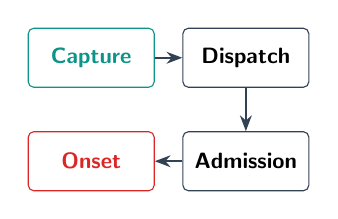
\begin{tikzpicture}[ev/.style={draw=figslate, fill=white, rounded corners=2pt, minimum width=1.6cm, minimum height=0.75cm, font=\footnotesize\bfseries}, ar/.style={-{Stealth[length=2mm]}, thick, figslate}]
        \node[ev, draw=figteal, text=figteal] (c) {Capture};
        \node[ev, right=0.35cm of c] (d) {Dispatch};
        \node[ev, below=0.55cm of d] (a) {Admission};
        \node[ev, left=0.35cm of a, draw=figred, text=figred] (o) {Onset};
        \draw[ar] (c) -- (d); \draw[ar] (d) -- (a); \draw[ar] (a) -- (o);
      \end{tikzpicture}\\[0.2cm]
      {\small Age runs from \textcolor{figteal}{\textbf{capture}}, when light or flux is transduced, to \textcolor{figred}{\textbf{onset}}, when current in the winding starts to move mass.}\\[0.15cm]
      \uncover<2->{\small $\tage = $ now $-$ capture time, on one hardware clock}
    \end{column}
  \end{columns}
  \mlsyscredit{The Physical Body, \S2.2.1 and \S2.2.2 (four boundary events). Photo: Dicklyon, CC BY-SA 4.0, Wikimedia Commons (Dash 8 propeller, Pixel 3 camera).}
  \note{[1.5 min] [CORE] The photo is real: a phone camera's rolling shutter reads the image row by row, and the propeller turned between the first row and the last. One frame is not one instant. Four events divide every interval from sensing to motion, and the book uses them throughout: capture (photons strike the sensor, or flux sweeps a Hall sensor), dispatch (perception publishes dated evidence to the proposer), admission (the permission path accepts a proposal built on it), onset (current in the stator starts to accelerate the joint). Step 2: the age that matters runs from capture to onset, and it means something only when camera, host, and drives read one clock, synchronized in hardware (IEEE 802.1AS). ENGAGE: where does a frame's age start for a rolling-shutter camera? (Expected: at a defined row's exposure midpoint; the frame-arrival interrupt comes later.) WARN: the age keeps growing after inference ends. LINK: Lecture 8 builds observation age stage by stage; today sets only the deadline it must meet.}
\end{frame}

\begin{frame}{Inference is about half of the age the joint acts on}
  \centering
  \mlsyssteps[width=\textwidth,height=5.0cm,keepaspectratio]{waterfall_step}{3}\\[0.05cm]
  \uncover<3->{\small Stage p99s sum to \val{p99_sum} ms; the end-to-end p99 is \val{p99_sys} ms. Measure the whole path.}
  \mlsyscredit{The Physical Body, table 1 (illustrative camera-to-joint grasp profile; median chain set equal to the stage sum) and Napkin Math 2.1 (p99.9 age \val{p999_sys} ms).}
  \note{[3 min] [CORE] The arm's wrist-camera grasp path, an illustrative profile from the chapter. Step 1: the number a benchmark reports, \val{st_backbone} ms for the vision backbone on an edge accelerator. It looks like a \val{backbone_hz} Hz loop (derived). Step 2: the whole path at the median: exposure and rolling-shutter readout \val{st_exposure} ms, PCIe transport and DMA \val{st_transport}, inference \val{st_backbone}, scheduling and the hand-off to the safety microcontroller \val{st_sched}, one EtherCAT cycle \val{st_fieldbus}, current rise \val{st_current}: \val{p50_sum} ms, of which inference is \val{backbone_pct} percent (derived). Step 3: the tail. The p99 age is \val{p99_sys} ms and the p99.9 age \val{p999_sys} ms. ENGAGE: the stage p99s sum to \val{p99_sum} ms, but the measured p99 is \val{p99_sys}. Why smaller? (Expected: stages rarely hit their worst at the same moment; the percentile of a sum is not the sum of percentiles.) WARN: coupled stages, sharing one memory controller, push the tail toward the sum, and a measured percentile is still not a hard real-time bound. Compressing the model from 30 to 10 ms (the chapter's fallacy) saves 20 ms that one 45 ms scheduling spike erases. FLEX: [CORE].}
\end{frame}

\begin{frame}{Does the grasp meet its \val{deadline} ms deadline?}
  \mlsysactivity{Predict}{3 min}
  \begin{columns}[c]
    \begin{column}{0.38\textwidth}
      \begin{mlsyscard}{mlsysaccent}
        \small\textbf{Given: mug on a conveyor}\\[0.05cm]
        Belt $v_{\max} = \val{belt}$ m/s; \val{tol_mm} mm tolerance, \val{err0_mm} mm spent\\[0.05cm]
        Freshness deadline:\\ $\tfresh \le \emax / v_{\max} = \textbf{\val{deadline} ms}$
      \end{mlsyscard}
      \vspace{0.1cm}
      {\small\choice{A}{both meet}\ \ \answerat{2}{B}{median only}\ \ \choice{C}{both miss}}
    \end{column}
    \begin{column}{0.60\textwidth}
      \centering
      \mlsyssteps[width=\textwidth,height=3.4cm,keepaspectratio]{mug_travel_step}{2}\\[0.1cm]
      \uncover<2->{\small Median: \val{mug_p50} mm of \val{emax_mm}. p99.9: \val{mug_tail} mm, \textbf{\textcolor{figred}{\val{mug_over} mm past}}.\\[0.05cm]
      \footnotesize A target twice as fast halves the deadline with no change in the pipeline.}
    \end{column}
  \end{columns}
  \mlsyscredit{The Physical Body, equation 1 and Napkin Math 2.1 (all values illustrative); mug travel derived in images/calcs.py.}
  \note{[3 min] [CORE] The freshness deadline turns a spatial tolerance into a time budget: the largest age a measurement of a moving target may reach before the target's motion alone spends the allowed error. The gripper tolerates \val{tol_mm} mm; the initial handle estimate spends \val{err0_mm}; \val{emax_mm} mm remain. At \val{belt} m/s, \val{emax_mm} mm lasts \val{deadline} ms. ENGAGE: one minute; with the previous slide's ages, vote. Step 2: B. At the \val{p50_sum} ms median the mug moves \val{mug_p50} mm, \val{mug_slack} mm inside. At the \val{p999_sys} ms p99.9 it moves \val{mug_tail} mm, \val{mug_over} mm past (derived). The model alone, \val{st_backbone} ms, fits with room to spare, which is why students who judge by the benchmark pick A. WARN: the deadline belongs to the task; neither the sensor nor the model sets it. A pipeline qualified on a slow belt misses on a faster one without any change in its own timing. When the base drives toward a person standing still, the same age is paid as blind travel, the first term of the stopping distance; that is the next segment. LINK: Lecture 3's mug evidence horizon starts from this deadline.}
\end{frame}

\begin{frame}{A stamp taken at publish time hides the first stages}
  \begin{columns}[c]
    \begin{column}{0.58\textwidth}
      \begin{logblock}[11]\bfseries
        \textcolor{midgray}{// cam2image.cpp, timerCallback()}\\
        \ind{4}cap \textgreater{}\textgreater{} frame;\\
        \ind{4}\textcolor{midgray}{...}\\
        \ind{4}if (show\_camera\_) \{\\
        \ind{6}cv::imshow("cam2image", frame);\\
        \ind{6}cv::waitKey(1);\\
        \ind{4}\}\\[0.1cm]
        \ind{4}std\_msgs::msg::Header header;\\
        \ind{4}header.frame\_id = frame\_id\_;\\
        \ind{4}\colorbox{figred!15}{header.stamp = this-\textgreater now();}\\
      \end{logblock}
    \end{column}
    \begin{column}{0.40\textwidth}
      \small The ROS~2 camera demo stamps each image when it builds the message.\\[0.2cm]
      \uncover<2->{Exposure, readout, transfer, and the display wait are already gone from the age.\\[0.2cm]}
      \uncover<3->{\textbf{\textcolor{figteal}{Fix:}} latch the stamp in hardware at frame start, on a synchronized clock.}
    \end{column}
  \end{columns}
  \mlsyscredit{ros2/demos, image\_tools/src/cam2image.cpp (rolling, commit f659270, 2026-09-14), lines 139 to 162, excerpt with lines omitted; Apache-2.0. The Physical Body, Systems Perspective 2.2.}
  \note{[2 min] [OPTIONAL] Real code from the ROS 2 demos repository, the camera publisher many students run first. Step 1: the callback grabs a frame from OpenCV, optionally shows it in a window and waits a millisecond, and only then sets the header's time stamp to the node's clock. Step 2: every stage before that line, exposure, readout, USB or MIPI transfer, driver queueing, and the display wait, is missing from any age computed from this stamp. The chapter calls this the publish timestamp anti-pattern. In the latency table it erases stages 1 to 4. ENGAGE: how much age would this hide on the grasp path of the waterfall slide? (Expected: at least the \val{st_exposure} ms of exposure and readout plus \val{st_transport} ms of transport.) Step 3: latch the stamp at the silicon, for example on the MIPI CSI-2 start-of-frame packet, on a clock synchronized by IEEE 802.1AS. WARN: this is a demo, and it is fine for a demo; the error is copying the pattern into a node whose stamps feed a permission path. FLEX: [OPTIONAL]. Land the segment: age runs from exposure to onset, and its tail sets the deadline's verdict.}
\end{frame}

% =============================================================================
% SECTION: STOPPING
% =============================================================================
\mlsysnote{[0.5 min] [CORE] Second budget: momentum. While the observation ages, the base keeps moving.}
\mlsysdivider{How fast may the base drive toward a person?}{The Physical Body, \S2.3}
\section{Stopping}

\begin{frame}{Two allowances bring the stop to \val{stop_full} mm of \val{d_clear_mm}}
  \centering
  {\small $\dstop = v\,\taudelay + \dfrac{v^2}{2\abrake} + \dloc + \dmargin \;\le\; \Dclear$}\\[0.05cm]
  \only<1|handout:0>{\mlsyskitfig[width=0.95\textwidth,height=3.9cm,keepaspectratio]{budget_bar_step2}}%
  \only<2-|handout:1>{\mlsyskitfig[width=0.95\textwidth,height=3.9cm,keepaspectratio]{budget_bar_step3}}\\[-0.2cm]
  \uncover<3->{\footnotesize Body-owned terms: \textbf{\val{stop_body} mm}. At \textbf{\val{v_fast} m/s} the same delay needs \textbf{\textcolor{figred}{\val{stop_fast} mm}}, \val{breach_fast} mm past the person.}
  \mlsyscredit{The Physical Body, eq.~2, Napkin Math 2.2; kit bar; calcs.py.}
  \note{[2.5 min] [CORE] Step 1: Lecture 1's bar, \val{rest_full} mm. Step 2: equation 2 adds the bar's third segment, two spatial allowances: the localization bound (\val{d_loc_mm} mm) and a protective clearance (\val{d_margin_mm} mm), space that must stay empty when the base is at rest. The stop now needs \val{stop_full} mm, \val{left_full} mm short of the person (derived). Step 3: the terms the body owns are braking \val{brake_mm} mm, the \val{overhead} mm of allowances, and \val{onset_mm} mm of travel during the \val{t_onset_ms} ms brake onset, \val{stop_body} mm. That leaves \val{left_body} mm for every delay the body does not own. The same delay at \val{v_fast} m/s needs \val{stop_fast} mm, \val{breach_fast} mm past the person. ENGAGE: from \val{v_drive} to \val{v_fast} m/s, which term grows most? (Expected: braking, from \val{brake_mm} to \val{brake_fast} mm; delay travel grows only from \val{blind_full} to \val{blind_fast} mm, because braking grows with the square of speed.) WARN: mass cancels from the braking distance for a given deceleration, but a heavier payload changes what deceleration is credible. The fixed overhead mirrors the ISO protective separation distance for robot arms. LINK: the chunk lease that spends part of the \val{left_body} mm is Lecture 4's.}
\end{frame}

\begin{frame}{Estimate: what does \val{v_fast} m/s cost in delay?}
  \mlsysactivity{Estimate}{2 min}
  \begin{columns}[T]
    \begin{column}{0.40\textwidth}
      \begin{mlsyscard}{mlsysaccent}
        \small\textbf{Given: the loaded base}\\[0.05cm]
        Drive limit \val{v_drive} m/s\\
        Proposed speed \val{v_fast} m/s\\
        $\abrake = \val{a_brake}$ m/s² (illustrative)
      \end{mlsyscard}
      \vspace{0.15cm}
      {\normalsize How many ms of extra delay at \val{v_drive} m/s cost the same distance?}
    \end{column}
    \begin{column}{0.56\textwidth}
      \small
      \wstep{2}{Braking at \val{v_fast} m/s: $\val{v_fast}^2/(2 \times \val{a_brake}) = \mathbf{\val{brake_fast}}$ mm, up \val{brake_growth}\%}
      \wstep{3}{Added braking: $\val{brake_fast} - \val{brake_mm} = \mathbf{\val{brake_added}}$ mm}
      \wstep{4}{Same distance as delay: $\val{brake_added} / \val{v_drive} = \textbf{\textcolor{mlsysaccent}{\val{dt_equiv} ms}}$}
      \uncover<4->{\footnotesize Each \val{dt_step} ms of delay at \val{v_drive} m/s costs \val{dt_step_mm} mm. A speed setpoint may rise only after the quadratic is solved again.}
    \end{column}
  \end{columns}
  \mlsyscredit{The Physical Body, Napkin Math 2.2, step 5 and systems insight; derived in images/calcs.py.}
  \note{[3 min] [OPTIONAL] ENGAGE: two minutes with a neighbor. Step 2: braking travel scales with v squared; \val{v_fast} squared over \val{two_a} is \val{brake_fast_m} m, \val{brake_growth} percent more than the \val{brake_mm} mm at the drive limit. Step 3: the step adds \val{brake_added} mm. Step 4: at \val{v_drive} m/s the base covers \val{v_mm_per_ms} mm per millisecond, so \val{brake_added} mm equals \val{dt_equiv} ms of added pre-brake delay (derived). A \val{speed_up_pct} percent faster setpoint costs more distance than a model that runs nearly \val{dt_equiv_s} s slower. Students who answer about 170 ms scaled braking linearly with speed. WARN: operators raise speed in a configuration file to raise throughput; the chapter's pitfall is that this changes the stopping budget quadratically and the thermal duty of every braking event. FLEX: [OPTIONAL]; if cut, state the \val{dt_equiv} ms result in one sentence on the previous slide.}
\end{frame}

\begin{frame}{The velocity ceiling falls as the clear distance shrinks}
  \centering
  \mlsyssteps[width=0.95\textwidth,height=4.9cm,keepaspectratio]{vceiling_step}{3}\\[0.05cm]
  {\small $\vmax = -\abrake\taudelay + \sqrt{(\abrake\taudelay)^2 + 2\abrake(\Dclear - \dloc - \dmargin)}$}
  \mlsyscredit{The Physical Body, equation 3 and Napkin Math 2.2 (\val{vmax_body} m/s body-only ceiling); other curves derived with the chapter's inputs; inspected floor $\mu = \val{mu_insp}$ (Napkin Math 2.3).}
  \note{[2.5 min] [CORE] Solving equation 2 for speed gives the velocity ceiling, equation 3: a speed limit that depends on the clear distance in front of the base, recomputed on the permission path as the scene changes. Step 1: with only the body's \val{t_onset_ms} ms brake onset, \val{d_clear_m} m allows \val{vmax_body} m/s, above the drive limit. Step 2: with Lecture 1's \val{tau_delay_ms} ms delay, \val{vmax_full} m/s; at the drive limit the base needs \val{dneed_full} m of clearance (derived). Step 3: on the inspected floor, friction \val{mu_insp}, deceleration falls to \val{a_insp} m/s² and the ceiling to \val{vmax_insp} m/s, below the drive limit (derived). ENGAGE: what happens to the ceiling when a person steps closer than \val{overhead} mm? (Expected: zero; and a moving base cannot reach zero at once, so a negative margin demands full braking.) WARN: lowering a speed setpoint changes only future motion. The present momentum stays, so the check must use the present state. LINK: Lecture 12 extends this ceiling with jerk ramps, a tracking bound, and a walking person.}
\end{frame}

\begin{frame}{Credible deceleration is the smallest of three ceilings}
  \begin{columns}[c]
    \begin{column}{0.27\textwidth}
      \centering\safeimg[width=\textwidth,height=2.6cm,keepaspectratio]{hub_motor_scooter.jpg}\\[0.02cm]
      {\footnotesize An opened hub motor}\\[0.1cm]
      {\footnotesize ZLLG10ASM800: \val{hub_tau_peak} N·m peak at \val{hub_i_peak} A, \val{hub_tau_rated} N·m rated}
    \end{column}
    \begin{column}{0.72\textwidth}
      \centering\safeimg[width=\textwidth,height=5.0cm,keepaspectratio]{decel_ceilings.pdf}\\[0.02cm]
      \uncover<2->{\small $\abrake \le \min(\mu g \varphi,\ \text{tip-over},\ \text{drive torque})$: peak current clears \val{a_brake_1} by \textbf{\val{torque_margin}\%}}
    \end{column}
  \end{columns}
  \mlsyscredit{The Physical Body, Napkin Math 2.3 (floor friction illustrative; ZLLG10ASM800 datasheet). Photo: Andrez1, CC BY-SA 4.0, Wikimedia Commons (an e-scooter hub motor).}
  \note{[2.5 min] [CORE] The photo is a kick-scooter hub motor with one side removed: copper coils on the fixed stator, magnets in the turning rim, no gearbox. The base brakes through two such motors of a larger industrial model, rated from its datasheet. Step 1: three ceilings, each owned by a different part of the machine. Traction: the floor supplies at most mu g times the share of weight on the driven wheels. The hub motors are rated for \val{load_pair} kg per pair, so at most \val{phi_max} of the \val{mass} kg; the dry floor then allows \val{a_dry} m/s², the inspected floor at most \val{a_insp}. Drive torque: \val{hub_kt} N·m/A times \val{hub_i_peak} A is \val{hub_tau_peak} N·m per wheel, \val{force} N at the floor; over at most \val{m_eff} kg including the rotating mass, at least \val{a_torque} m/s². With the current limit at the rated \val{hub_i_rated} A, \val{a_rated}. Tip-over: the center of gravity has not been measured, and extending the arm changes it. Step 2: the credible deceleration is the minimum. ENGAGE: an engineer lowers the drive's current limit to protect the windings. Which ceiling moves, and does any software change? (Expected: drive torque falls below \val{a_brake_1} with no code change.) WARN: the \val{a_brake} m/s² rests on peak current, a dry floor, and an unmeasured center of gravity. FLEX: [CORE]. Land the segment.}
\end{frame}

% =============================================================================
% SECTION: ACTUATORS
% =============================================================================
\mlsysnote{[0.5 min] [CORE] Land the segment aloud: the stop is linear in delay and quadratic in speed, and its deceleration is the smallest of three separately owned ceilings. Third budget: can the drive deliver the torque that deceleration needs?}
\mlsysdivider{Does an acknowledged torque command deliver torque?}{The Physical Body, \S2.4}
\section{Actuators}

\begin{frame}{True or false: a torque step arrives at once?}
  \mlsysactivity{Concept question}{2 min}
  \centering
  {\normalsize ``A policy that writes a torque setpoint gets that torque at the next tick.''}\\[0.25cm]
  {\normalsize\choice{A}{true}\qquad\answerat{2}{B}{false}}\\[0.3cm]
  \begin{columns}[T]
    \begin{column}{0.48\textwidth}
      \small
      \uncover<2->{$\tau = \Kt\, i$, and the winding resists change:\\ $L\, di/dt = V - R\,i - E_{\text{bemf}}$\\[0.1cm]
      Hub motor: $L/R = \val{tau_e}$ ms; rise to \val{hub_i_peak} A in about \val{t_ramp} ms on \val{v_low} V}
    \end{column}
    \begin{column}{0.48\textwidth}
      \small
      \uncover<3->{At \val{v_drive} m/s the back-EMF is \textbf{\val{bemf} V}.\\[0.05cm]
      Braking at \val{hub_i_peak} A needs \val{v_brake} V.\\
      Driving at \val{hub_i_peak} A needs \textbf{\textcolor{figred}{\val{v_drive_need} V}}, more than a \val{v_low} V pack.}
    \end{column}
  \end{columns}
  \mlsyscredit{The Physical Body, \S2.4.2 and Napkin Math 2.3, step 4 (ZLLG10ASM800: \val{l_line} mH, \val{r_line} $\Omega$, \val{ke_hub} V/rpm line to line); fallacy from \S2.9. Derived in images/calcs.py.}
  \note{[2.5 min] [CORE] The chapter's fallacy, as a vote. ENGAGE: 30 seconds, hands up. Step 2: false. Torque is a current, and the winding is a coil, so current cannot jump. By Kirchhoff's law around the winding, the supply covers the resistive drop, the inductive voltage, and the back-EMF, the voltage the spinning motor generates against its own supply. The hub motor's electrical time constant is \val{tau_e} ms; driving full voltage into it from rest, current reaches \val{hub_i_peak} A in about \val{t_ramp} ms, \val{ramp_pct} percent of the \val{t_onset_ms} ms brake onset (derived; optimistic, since resistance slows the ramp). On this machine the rise is fast enough. Step 3: speed binds. At \val{v_drive} m/s the wheel turns \val{rpm_drive} rpm and generates \val{bemf} V. Braking current flows with the back-EMF and needs only \val{v_brake} V at the terminals; driving current fights it and needs \val{v_drive_need} V, which a depleted \val{v_low} V pack cannot supply. WARN: a simulator that applies commanded torque instantly teaches a policy actions the drive cannot deliver; a learned actuator model identified on hardware (ANYmal, Hwangbo et al. 2019) closes that gap, and Lecture 6 owns the reality gap.}
\end{frame}

\begin{frame}{The configured current limit caps delivered torque}
  \begin{columns}[c]
    \begin{column}{0.50\textwidth}
      \centering
      {\large $\tauoutmax = \etagear\, \Ngear\, \Kt\, \Imax$}\\[0.3cm]
      \small A drive can clamp current to $\Imax$ and still acknowledge every packet.\\[0.25cm]
      \uncover<2->{\begin{mlsyscard}{figred}\small Hub motor, $\Ngear = 1$:\\ \val{hub_i_peak} A gives \val{hub_tau_peak} N·m per wheel; \val{hub_i_rated} A gives \val{hub_tau_rated} N·m. The setpoint says neither.\end{mlsyscard}}
    \end{column}
    \begin{column}{0.48\textwidth}
      \centering\safeimg[width=\textwidth,height=3.4cm,keepaspectratio]{volt_need.pdf}\\[0.15cm]
      \uncover<3->{\small The permission path reads \textbf{measured phase current} and the saturation flag on every stop.}
    \end{column}
  \end{columns}
  \mlsyscredit{The Physical Body, equation 4, \S2.4.1 and \S2.4.2, Napkin Math 2.3; ZLLG10ASM800 datasheet values as cited there.}
  \note{[2 min] [CORE] Equation 4: the delivered torque ceiling is the gear efficiency times the ratio times the torque constant times the inverter's current limit. Step 1: in a computer, a target either executes an instruction or raises a fault. A motor drive can clamp current at its limit while it keeps acknowledging setpoints on the bus, so a 50 N·m request can quietly deliver 25. Step 2: on the base, the limit set at the \val{hub_i_peak} A peak gives \val{hub_tau_peak} N·m per wheel; at the \val{hub_i_rated} A rated current, \val{hub_tau_rated} N·m. The figure repeats the voltage side. Braking needs \val{v_brake} V, driving \val{v_drive_need} V against a \val{v_low} V pack. Step 3: so the safety path reads measured current and the drive's saturation flag; an acknowledgement proves only that the packet arrived. ENGAGE: a firmware update changes the default current limit. Which record must be recomputed? (Expected: the stopping limit record, because its deceleration rests on that limit.) WARN: dead time in the inverter distorts delivered torque most at low speed, exactly where fine contact force is commanded; verify torque on a dynamometer. FLEX: [CORE].}
\end{frame}

\begin{frame}{Gearing multiplies torque by $\Ngear$ and rotor inertia by $\Ngear^2$}
  \begin{columns}[c]
    \begin{column}{0.60\textwidth}
      \centering\safeimg[width=\textwidth,height=5.6cm,keepaspectratio]{accel_ratio.pdf}
    \end{column}
    \begin{column}{0.38\textwidth}
      \small Reflected rotor inertia $= \Ngear^2 \Jrotor$\\[0.15cm]
      \uncover<2->{A \val{rotor_g} g rotor through \val{n_gear}:1 acts like an \textbf{\val{fly_kg} kg} flywheel of \val{fly_cm} cm radius at the joint.\\[0.15cm]}
      \uncover<3->{Acceleration peaks where $\Ngear^2 \Jrotor = \Jload$:\\ $N^* = \sqrt{\Jload/\Jrotor} \approx \textbf{\val{n_star}}$}
    \end{column}
  \end{columns}
  \mlsyscredit{The Physical Body, \S2.4.3, definition 2.3, equation 5 (illustrative rotor and link inertias); curve $2x/(1+x^2)$, $x = \Ngear/N^*$, derived in images/calcs.py.}
  \note{[3 min] [CORE] The curve uses an illustrative rotor of $\val{j_rotor_mant} \times 10^{-6}$ and a link of $\val{j_load_mant} \times 10^{-3}$ kg·m². Step 1: a gearbox makes the motor turn N times faster than the joint, so its torque at the joint is N times larger, but its rotor's kinetic energy grows with the square of speed. Seen from the joint, the rotor's inertia is N squared times larger; the book calls this reflected rotor inertia. Step 2: through \val{n_gear}:1 a \val{rotor_g} g rotor has \val{j_ref} kg·m² at the joint, the inertia of an \val{fly_kg} kg solid disk \val{fly_cm} cm in radius (derived). An impact must stop that flywheel through the gear teeth before current can be cut. Step 3: the curve. Joint acceleration is N times motor torque over the link inertia plus N squared times rotor inertia. Below N* = \val{n_star} more gearing helps (torque-limited); above it the motor spends its torque spinning its own rotor. At \val{n_gear}:1 the joint keeps \val{accel_pct} percent of the highest acceleration (derived). ENGAGE: why do real arms often choose ratios below N*? (Expected: lower ratios protect teeth from shock, keep the joint backdrivable, and raise top speed; N* maximizes acceleration only.) WARN: Lecture 11 uses these limits to time trajectories. FLEX: [CORE].}
\end{frame}

\begin{frame}{A strain wave gear adds a spring between motor and link}
  \begin{columns}[c]
    \begin{column}{0.49\textwidth}
      \centering\safeimg[width=\textwidth,height=4.3cm,keepaspectratio]{fig02_real_strain_wave_gear.jpg}\\[0.02cm]
      {\footnotesize Wave generator, flexspline cup, circular spline}
    \end{column}
    \begin{column}{0.49\textwidth}
      \centering\safeimg[width=\textwidth,height=3.4cm,keepaspectratio]{fig02_real_broken_gear_tooth.jpg}\\[0.02cm]
      {\footnotesize A spur gear tooth broken at its root (NASA, 1974)}\\[0.12cm]
      \uncover<2->{\small The motor encoder sees smooth rotation while the flexspline winds up and the link lags.}
    \end{column}
  \end{columns}
  \mlsyscredit{The Physical Body, figures 3 and 4. Photos: Pieceofmetalwork, CC BY-SA 4.0, Wikimedia Commons; Martin Brown, NASA Glenn Research Center, NARA 17417956, public domain.}
  \note{[2 min] [OPTIONAL] Left: a disassembled strain wave gear, sold as the Harmonic Drive. The elliptical wave generator flexes the thin toothed cup inside a rigid ring with two more teeth, so one stage gives 50:1 to 160:1 with near-zero backlash. The flexing that makes the ratio possible is also a torsional spring. Step 2: the motor-side encoder reports smooth tracking while the flexspline twists and the link lags by a load-dependent angle. In ordinary gears, backlash adds lost motion at every reversal, and a controller hunting across that gap settles into a limit cycle, a fixed-amplitude oscillation that adds a tooth impact every cycle. Right: the end state of repeated shock, a tooth broken at its root, from NASA gear research. ENGAGE: what sensor exposes the windup the motor encoder hides? (Expected: a load-side encoder or a joint torque sensor; the running machine's arm puts a torque sensor in each joint.) WARN: static payload ratings do not size a gear; impact loads do. FLEX: [OPTIONAL].}
\end{frame}

\begin{frame}{For one motor, holding heat times reflected inertia is fixed}
  \begin{columns}[c]
    \begin{column}{0.30\textwidth}
      \centering\safeimg[width=\textwidth,height=4.2cm,keepaspectratio]{franka_panda_arm.jpg}\\[0.02cm]
      {\footnotesize Franka Emika Panda, the arm class}
    \end{column}
    \begin{column}{0.68\textwidth}
      \small Hold \val{tau_out} N·m through a strain wave gear with one frameless motor (TQ ILM 70x18, peak \val{motor_peak} N·m)\\[0.15cm]
      \begin{tabular}{@{}rrrr@{}}\toprule
        \textbf{Ratio} & \textbf{Motor torque} & \textbf{Copper loss} & \textbf{Reflected inertia}\\\midrule
        \val{n_high}:1 & \val{tm_high} N·m & \val{loss_high} W & \val{jr_high} kg·m²\\
        \val{n_joint}:1 & \val{tm_joint} N·m & \val{loss_joint} W & \val{jr_joint} kg·m²\\
        \uncover<2->{\val{n_qdd}:1} & \uncover<2->{\textcolor{figred}{\textbf{\val{tm_qdd} N·m}}} & \multicolumn{2}{l}{\uncover<2->{\textcolor{figred}{\val{qdd_over}$\times$ the motor's peak}}}\\\bottomrule
      \end{tabular}\\[0.2cm]
      \uncover<3->{$\Ploss \times \Ngear^2 J_{\text{in}} = \dfrac{\tau_{\text{out}}^2 J_{\text{in}}}{\etagear^2 K_m^2}$: the ratio moves the joint along the trade; only the motor sets it.}
    \end{column}
  \end{columns}
  \mlsyscredit{The Physical Body, equation 6, Napkin Math 2.4 (TQ ILM 70x18 and CSG-25 datasheets; \val{eta} efficiency illustrative). Photo: Ims, CC BY-SA 4.0, Wikimedia Commons.}
  \note{[2.5 min] [CORE] The running machine's arm is a seven-joint, torque-sensing arm of the Franka Panda's class. Franka does not publish its joint motors, so the chapter uses a sourced stand-in: a TQ ILM 70x18 frameless motor (motor constant \val{km} N·m per square root of watt) driving a CSG-25 strain wave gear, holding the arm's \val{tau_out} N·m at \val{eta_pct} percent efficiency. Step 1: at \val{n_joint}:1 the motor supplies \val{tm_joint} N·m and burns \val{loss_joint} W; at \val{n_high}:1, a quarter of the heat, \val{loss_high} W, and \val{loss_ratio_words} times the reflected inertia. Step 2: at a quasi-direct-drive \val{n_qdd}:1 the motor would need \val{tm_qdd} N·m, \val{qdd_over} times its peak; no current can hold the load. Step 3: copper loss falls as 1 over N squared and reflected inertia rises as N squared, so their product, \val{product} W·kg·m² here (derived), does not depend on the ratio. ENGAGE: how does MIT's Cheetah get a backdrivable low-ratio joint? (Expected: a much larger motor, a higher motor constant squared over input inertia.) WARN: a high-ratio arm recovers contact sensitivity by measuring torque at the output, which the Panda does. FLEX: [CORE]. Land the segment.}
\end{frame}

% =============================================================================
% SECTION: HEAT AND POWER
% =============================================================================
\mlsysnote{[0.5 min] [CORE] Land the segment aloud: a setpoint is a current request that voltage, the current limit, and the gear ratio shape; the ratio trades heat for inertia. Every ampere of that current becomes heat in copper and a draw on the shared bus.}
\mlsysdivider{Where does the energy go when the body works?}{The Physical Body, \S2.5, \S2.6, \S2.8.2}
\section{Heat and Power}

\begin{frame}{A joint holding still turns every watt into heat}
  \begin{columns}[c]
    \begin{column}{0.40\textwidth}
      \centering\safeimg[width=\textwidth,height=3.4cm,keepaspectratio]{fig02_real_burnt_motor_stator.jpg}\\[0.02cm]
      {\footnotesize A stator that failed from overheating}\\[0.15cm]
      \small $\Ploss = i^2 R = (\tau/\Kt)^2 R$\\ Twice the torque, four times the heat
    \end{column}
    \begin{column}{0.58\textwidth}
      \centering\safeimg[width=\textwidth,height=4.6cm,keepaspectratio]{envelope.pdf}\\[0.02cm]
      \uncover<2->{\small Heat rejection sets continuous torque; peak is \textbf{\val{peak_over_rated}$\times$} continuous}
    \end{column}
  \end{columns}
  \mlsyscredit{The Physical Body, \S2.5.1, equation 7, figure 6a (TQ ILM 70x18 datasheet torques; voltage limit from the chapter). Photo: K.~Kudelina, CC BY 4.0, Wikimedia Commons (book figure 5).}
  \note{[2 min] [CORE] Holding a mass still does no mechanical work, but a motor holds it with current, and current through copper makes heat, so the loss grows with torque squared. Left: an opened stator that failed from overheating; the damage sits in the windings and the insulation between them, where this model puts the heat. Right: the stand-in arm motor. Step 1: the gray region is S1, continuous duty, up to \val{motor_rated} N·m; the amber region is S3, bursts, up to the \val{motor_peak} N·m peak; the red line is the voltage limit, where back-EMF uses up the supply, from \val{n0_rpm} rpm at no load to \val{n_pk_rpm} at peak torque. Step 2: continuous torque is about a third of peak, \val{peak_over_rated} times less (derived), because the rate at which heat leaves sets it, while the drive could push three times more. ENGAGE: the datasheet rating comes from an open motor on a large heat sink at \val{t_catalog} °C. What happens in a sealed arm at \val{t_amb} °C? (Expected: less; the chapter's pitfall computes \val{derate_ambient} percent lost to ambient alone and \val{derate_both} percent if the thermal resistance doubles.) FLEX: [CORE].}
\end{frame}

\begin{frame}{How long can a hot joint hold a burst?}
  \mlsysactivity{Predict}{3 min}
  \begin{columns}[c]
    \begin{column}{0.30\textwidth}
      \begin{mlsyscard}{mlsysaccent}\small
        \textbf{Given:} \val{burst_x}$\times$ rated current, \val{p_burst} W\\[0.03cm]
        $\tau_{\text{th}} = \val{tau_th}$ s, \val{t_amb} °C ambient\\[0.03cm]
        Limit \textcolor{figred}{\val{t_limit} °C} (Class F)\\[0.03cm]
        Cold start: \textbf{\val{t_cold} s}
      \end{mlsyscard}
      \vspace{0.1cm}
      {\small Starting hot, at \val{t_eq} °C?}\\[0.08cm]
      {\small\choice{A}{\val{t_cold_0} s}\ \answerat{2}{B}{\val{t_hot_0} s}\ \choice{C}{8 s}}
    \end{column}
    \begin{column}{0.68\textwidth}
      \centering
      \mlsyssteps[width=\textwidth,height=4.3cm,keepaspectratio]{burst_step}{2}\\[0.05cm]
      \uncover<2->{\small Heat-soaked: \textbf{\textcolor{figamber}{\val{hot_cut}\% less time}}. History spends peak torque.}
    \end{column}
  \end{columns}
  \mlsyscredit{The Physical Body, Napkin Math 2.5 (TQ ILM 70x18; thermal capacitance \val{c_th} J/K and resistance \val{theta_burst} K/W illustrative) and figure 6b; derived in images/calcs.py.}
  \note{[3 min] [CORE] A first-order thermal model of the stand-in joint: \val{c_th} J/K of thermal capacitance and \val{theta_burst} K/W to a \val{t_amb} °C enclosure, a \val{tau_th} s time constant (thermal values illustrative). \Val{burst_words} times rated current dissipates \val{heat_words} times the heat, \val{p_burst} W, heading for \val{t_inf} °C, far past the \val{t_limit} °C rating of Class F insulation. From ambient the winding reaches \val{t_limit} °C after \val{t_cold} s. ENGAGE: one minute; vote. Step 2: B. After running at rated current the winding starts at \val{t_eq} °C and reaches the limit in \val{t_hot} s, \val{hot_cut} percent less time (derived). Students who pick A treat peak torque as a fixed rating; students who pick C overestimate how fast a \val{tau_th} s mass heats. WARN: these horizons are optimistic: the copper hotspot runs ahead of this lumped temperature, and a thermistor on the case lags further. The class temperature marks no cliff; insulation ages as a chemical reaction whose rate grows exponentially with temperature, so the record counts time at temperature. A \val{burst_on} s burst every \val{burst_period} s passes the average-power screen (\val{duty_pct} percent duty) yet peaks at \val{t_peak} °C, above the \val{t_ceiling} °C working ceiling. LINK: Lecture 13 owns thermal throttling of compute.}
\end{frame}

\begin{frame}{A stalled elbow settles at \val{t_wind_0} °C unless it is derated}
  \begin{columns}[T]
    \begin{column}{0.42\textwidth}
      \begin{mlsyscard}{mlsysaccent}\small
        \textbf{Given:} elbow holds \val{tau_out} N·m at stall, \val{n_joint}:1, \val{eta}\\[0.03cm]
        $\Kt = \val{kt_motor}$ N·m/A; \val{r_loss} $\Omega$ at \val{t_ref} °C\\[0.03cm]
        \val{theta_stall} K/W (illustrative), \val{t_amb} °C\\[0.03cm]
        Copper: $+\val{alpha_pct}\%$ per K
      \end{mlsyscard}
    \end{column}
    \begin{column}{0.56\textwidth}
      \small
      \wstep{1}{Stall current \val{i_stall} A; \val{loss_joint} W cold}
      \wstep{2}{Resistance rises with heat; feedback factor \val{gain} $<$ 1, so it settles}
      \wstep{3}{Settles at \textbf{\textcolor{figred}{\val{t_wind} °C}}, far past \val{t_limit} °C}
      \wstep{4}{Sustainable: \val{i_sus} A, \textbf{\val{tau_sus} N·m}, a \val{derating}\% derating}
      \uncover<4->{\footnotesize Holding more needs a brake or counterweight in the admitted premise.}
    \end{column}
  \end{columns}
  \mlsyscredit{The Physical Body, Napkin Math 2.6 (TQ ILM 70x18 stand-in; thermal resistance illustrative); derived in images/calcs.py.}
  \note{[2 min] [OPTIONAL] At stall the motor does no work, so every watt becomes heat, and copper's resistance rises \val{alpha_pct} percent per kelvin, so the heat grows with the temperature it causes. Step 1: \val{tau_out} N·m through \val{n_joint}:1 at \val{eta_pct} percent efficiency is \val{tm_joint} N·m at the motor, \val{i_stall} A, \val{loss_joint} W cold. Step 2: the steady rise satisfies a linear equation whose loop gain here is \val{gain}; below 1 it settles, at or above 1 the fixed-current model has no equilibrium, thermal runaway. Step 3: it settles at a \val{rise_ss} K rise, \val{t_wind} °C. Step 4: at \val{t_limit} °C the winding resistance is \val{r_hot} ohm; the \val{p_sus} W the installation can reject allows \val{i_sus} A, \val{tau_sus} N·m, \val{derating} percent less (all derived). ENGAGE: why is cutting holding current not a safe response? (Expected: a gravity-loaded arm then falls; the load must move to a brake first.) FLEX: [OPTIONAL].}
\end{frame}

\begin{frame}{Compute and drives share one power rail, and a step sags it}
  \begin{columns}[c]
    \begin{column}{0.28\textwidth}
      \centering\safeimg[width=\textwidth,height=3.2cm,keepaspectratio]{erflex_mir250_ur16e.jpg}\\[0.02cm]
      {\footnotesize MiR250-class base: \val{v_full} V full, \val{v_low} V depleted}
    \end{column}
    \begin{column}{0.70\textwidth}
      \small Shared rail: inference and drives draw \textbf{\val{i_step} A} through \val{r_bus_mohm} m$\Omega$\\[0.05cm]
      \centering\safeimg[width=\textwidth,height=2.9cm,keepaspectratio]{bus_sag.pdf}\\[0.05cm]
      \raggedright
      \uncover<2->{$\val{i_step} \times \val{r_bus_ohm} = \val{sag}$ V sag leaves a depleted pack at \textbf{\val{v_sag_low} V}, \val{v_margin} V above lockout\\[0.05cm]}
      \uncover<3->{\footnotesize Sustained screen only; the transient dips lower.}
    \end{column}
  \end{columns}
  \mlsyscredit{The Physical Body, Napkin Math 2.7 (MiR250 pack envelope; DDR-240 \val{v_uvlo} V lockout; \val{r_bus_mohm} m$\Omega$ and \val{i_step} A illustrative). Photo: Auledas, CC BY 4.0, Wikimedia Commons.}
  \note{[2.5 min] [CORE] The running machine's pack has the voltage envelope of the MiR250 base in the photo: \val{v_full} V full, \val{v_low} V depleted. One 48 V bus feeds the wheel drives, the arm drives, and a 48-to-24 V converter for the application processor, which shuts off below \val{v_uvlo} V. Step 1: an obstacle response asks for fresh inference and hard acceleration at once: \val{i_drive} A for the drives plus \val{i_compute} A for a \val{p_soc} W processor, \val{i_step} A. Step 2: through \val{r_bus_mohm} milliohms of cells, harness, and switches, \val{sag} V of sustained sag. A full pack sits at \val{v_sag_full} V; a depleted one at \val{v_sag_low} V, \val{v_margin} V above lockout. It would take a \val{i_cross} A step to spend the \val{v_headroom} V (derived). Step 3: this screens only the settled drop. ENGAGE: the same robot on a cold morning, five years later. What changed? (Expected: cell resistance rose, so the same step sags further.) WARN: testing compute and motors separately never sees the coincident step; the chapter's fallacy treats them as independent rails. If the safety microcontroller shares this rail, a brownout resets it with the base moving. FLEX: [CORE].}
\end{frame}

\begin{frame}{Estimate: where does a stop's \val{ke} J go?}
  \mlsysactivity{Estimate}{2 min}
  \begin{columns}[T]
    \begin{column}{0.36\textwidth}
      \begin{mlsyscard}{mlsysaccent}\small
        \textbf{Given:} \val{mass} kg at \val{v_drive} m/s, full \val{v_full} V pack refuses charge\\[0.03cm]
        \val{regen_pct}\% returns (illustrative)\\[0.03cm]
        \val{c_bus} $\mu$F bus; \val{t_stop} ms stop
      \end{mlsyscard}
      \vspace{0.1cm}
      \small
      \wstep{2}{$\val{regen_frac} \times \val{ke} = \val{e_regen}$ J}
      \wstep{3}{$V = \sqrt{\val{v_full}^2 + 2E/C} = \textbf{\textcolor{figred}{\val{v_final} V}}$}
    \end{column}
    \begin{column}{0.62\textwidth}
      \centering\uncover<3->{\safeimg[width=\textwidth,height=3.7cm,keepaspectratio]{bus_surge.pdf}}\\[0.1cm]
      \raggedright\small
      \wstep{4}{Chopper peak power $2E/t = \val{p_peak}$ W; resistor $\le \val{v_clamp}^2/\val{p_peak} = $ \textbf{\val{r_max}}~$\Omega$}
    \end{column}
  \end{columns}
  \mlsyscredit{The Physical Body, equation 10 and Napkin Math 2.7 (MEAN WELL DDR-240 \val{v_conv_max} V input maximum; \val{v_switch} V switch rating); derived in images/calcs.py.}
  \note{[3 min] [CORE] ENGAGE: two minutes in pairs: where does the energy go if the battery refuses it? The worst case is a full pack, when the battery management system blocks charge. Step 2: \val{regen_pct} percent of \val{ke} J returns, \val{e_regen} J (illustrative share). Step 3: if only the \val{c_bus} microfarad bus capacitors take it, the voltage rises to \val{v_final} V, past the converter's \val{v_conv_max} V input limit and the \val{v_switch} V switch rating (derived). Students usually expect a few volts; the capacitor holds very little energy between \val{v_full} and \val{v_clamp} V, \val{e_clamp} J. Step 4: a brake chopper switches a resistor across the bus at a \val{v_clamp} V clamp. Speed falls linearly in a constant-deceleration stop, so regenerated power falls linearly from twice its average: \val{p_peak} W. At \val{v_clamp} V the resistor must be at most \val{r_max} ohm; a \val{r_cand} ohm, \val{p_cand} kW part is the chapter's choice. WARN: the capacitor-only number is a screen; the chopper's pulse energy, repetition, and cooling still need qualification. Land: acceleration needs a supply that holds; deceleration needs a sink.}
\end{frame}

\begin{frame}{Cutting power leaves a joint in one of three states}
  \begin{columns}[c]
    \begin{column}{0.54\textwidth}
      \centering\safeimg[width=\textwidth,height=3.8cm,keepaspectratio]{phase_short.pdf}\\[0.02cm]
      {\footnotesize Free coast: no torque. Spring brake: engages after \val{brake_min} to \val{brake_max} ms. Phase short: peaks at \val{rpm_short} rpm.}
    \end{column}
    \begin{column}{0.44\textwidth}
      \centering\safeimg[width=\textwidth,height=2.0cm,keepaspectratio]{supercapacitor_modules.jpg}\\[0.02cm]
      {\footnotesize Supercapacitor modules and cells}\\[0.15cm]
      \raggedright\small
      \uncover<2->{Permission rail: \val{c_hold} F from \val{v_hold_hi} to \val{v_hold_lo} V holds \textbf{\val{e_hold} J}, \textbf{\val{t_hold} s} at \val{p_perm} W.\\[0.05cm]
      \footnotesize It keeps the checks alive; it does not power a braking drive.}
    \end{column}
  \end{columns}
  \mlsyscredit{The Physical Body, \S2.6.2 and \S2.8.2 (hub motor \val{r_line} $\Omega$, \val{l_line} mH, \val{pole_pairs} pole pairs; hold-up values from the chapter). Photo: Sechsa, CC0, Wikimedia Commons.}
  \note{[2 min] [OPTIONAL] Removing power changes the joint's state and does not return it to safety. Step 1: three unpowered states. Free coast: no torque, gravity and momentum continue. A spring-applied brake engages after \val{brake_min} to \val{brake_max} ms of coil decay. Phase short: shorting the windings turns back-EMF into braking torque, which grows with speed until the winding's reactance limits the current; for the hub motors the torque peaks at \val{rpm_short} rpm of the wheel, above the \val{rpm_drive} rpm drive limit, so it still rises across the base's range (derived). A fast high-ratio joint motor has no such guarantee. Step 2: the running machine isolates the permission logic, fieldbus transceivers, and brake-release coils on a separate, reverse-blocked rail held up by a \val{c_hold} F bank: \val{e_hold} J between \val{v_hold_hi} and \val{v_hold_lo} V, \val{t_hold} s at \val{p_perm} W (derived), against a \val{t_stop} ms stop plus \val{brake_max} ms brake. ENGAGE: does a held-up permission rail guarantee the \val{a_brake} m/s² stop? (Expected: no; a powered stop also needs the drive rail and an energy sink.) LINK: Lecture 12 picks the fallback state; Lecture 13 owns compute throttling, which stretched the navigation backbone from \val{t_backbone} to \val{t_throttled} ms, \val{d_throttle} mm of blind travel.}
\end{frame}

% =============================================================================
% SECTION: LIMITS
% =============================================================================
\mlsysnote{[0.5 min] [CORE] Land the segment aloud: heat arrives in seconds and leaves in minutes, and the bus must hold during a coincident step and absorb a stop. Every limit today came with conditions. What makes a number usable by the permission path?}
\mlsysdivider{When may the permission path rely on a number?}{The Physical Body, \S2.7 and \S2.8}
\section{Limits}

\begin{frame}{A limit holds only under the conditions of its test}
  \begin{columns}[c]
    \begin{column}{0.48\textwidth}
      \centering\safeimg[width=\textwidth,height=4.0cm,keepaspectratio]{fig02_real_motor_dyno_bench.jpg}\\[0.02cm]
      {\footnotesize Instrumented propulsion test stand, NASA Armstrong, 2016}
    \end{column}
    \begin{column}{0.50\textwidth}
      \small Every number falls in one of five evidence categories:\\[0.1cm]
      \begin{tabular}{@{}ll@{}}
        \textbf{\textcolor{figgreen}{measured}} & \textbf{\textcolor{figgreen}{derived}} from measurements\\
        \textcolor{figamber}{datasheet} & \textcolor{figred}{illustrative}\quad \textcolor{figslate}{chosen}
      \end{tabular}\\[0.2cm]
      \uncover<2->{Only measured and derived values can support a safety margin.\\[0.1cm]
      \footnotesize Record payload, ambient, supply, enclosure, firmware, and concurrent compute.}
    \end{column}
  \end{columns}
  \mlsyscredit{The Physical Body, \S2.7.1 and \S2.7.3. Photo: Lauren Hughes, NASA Armstrong Flight Research Center, AFRC2016-0100-05, public domain (book figure 7).}
  \note{[2 min] [OPTIONAL] A test stand measures what a datasheet only asserts, on the assembled drive under stated conditions. Dynamometer tests give the torque and back-EMF constants, the electrical time constant (with a small voltage step, because the full \val{v_low} V across the hub motor's \val{r_line} ohm would drive \val{i_full_step} A), the installed thermal resistance, and backdrive friction. Step 1: the five categories decide how far a decision may rely on a number. Step 2: only a measurement, or a value derived from measurements through a stated model, can support a margin. The \val{a_torque} m/s² drive ceiling, computed from datasheet values, keeps datasheet standing; the \val{d_margin_mm} mm clearance is chosen and binds only once checked against a measured uncertainty. ENGAGE: classify the \val{a_brake} m/s² credible deceleration. (Expected: illustrative.) WARN: measurement changes the plant. A shunt drops voltage, and a probe changes a heat path. A clean campaign of \val{n_stops} stops bounds the failure rate only below about 1 in \val{one_in} at \val{conf_pct} percent confidence; Lecture 7 owns that bound. FLEX: [OPTIONAL].}
\end{frame}

\begin{frame}{A limit record carries six elements with its value}
  \centering\footnotesize\setlength{\parskip}{0pt}
  \renewcommand{\arraystretch}{1.35}
  \begin{tabular}{@{}ll@{}}\toprule
    \textbf{Element} & \textbf{Credible deceleration of the running machine}\\\midrule
    Value & \val{a_brake} m/s², the credible low tail of loaded stops; no samples yet\\
    \uncover<2->{Conditions} & \uncover<2->{$\le$ \val{mass} kg; $\mu\varphi \ge \val{mu_min}$, never the inspected floor; \val{hub_i_peak} A current limit; tip-over unmeasured}\\
    \uncover<3->{Uncertainty} & \uncover<3->{Not established: what is unknown about the measurement}\\
    \uncover<3->{Margin} & \uncover<3->{None justified yet; margin is clearance defended against the unknown}\\
    \uncover<4->{\textbf{\textcolor{figred}{Detector}}} & \uncover<4->{\textbf{\textcolor{figred}{Commanded against measured deceleration (encoders, BMI088 IMU), every stop}}}\\
    \uncover<4->{Provenance} & \uncover<4->{Illustrative; to be replaced by loaded stopping trials}\\\bottomrule
  \end{tabular}\par\vspace{0.2cm}
  \small\uncover<4->{A number governs admission only with its conditions, evidence, and detector.}
  \mlsyscredit{The Physical Body, \S2.7.3 and table 3 (credible deceleration column), abridged.}
  \note{[2.5 min] [CORE] The limit record, the one record this lecture adds to the record chain. Step 1: the value, and how it was obtained; here it is still a placeholder. Step 2: the conditions under which it holds: payload, floor friction times wheel load share, the drive's current limit, tire wear, and a tip-over geometry nobody has measured. Each segment today produced one of these conditions. Step 3: uncertainty and margin, the pair students conflate. Uncertainty describes the measurement (noise, instrument tolerance, calibration drift); margin is the clearance the machine defends against it. Step 4: the detector, the runtime check that notices when operation leaves the conditions, and the provenance, the evidence category. ENGAGE: name the condition that a lowered current limit, the inspected floor, and an extended arm would each violate. (Expected: the \val{hub_i_peak} A limit; mu times phi at least \val{mu_min}; the unmeasured tip-over geometry.) WARN: records lapse as the machine ages: batteries gain resistance, gearboxes gain backlash, enclosures lose cooling. LINK: Lecture 4's handoff record carries each limit record to the permission path.}
\end{frame}

\begin{frame}{Diagnose: which element did Schiaparelli lack?}
  \mlsysactivity{Diagnose}{2 min}
  \begin{columns}[c]
    \begin{column}{0.38\textwidth}
      \centering\safeimg[width=\textwidth,height=2.8cm,keepaspectratio]{schiaparelli_ctx_before_after.jpg}\\[0.1cm]
      \begin{mlsyscard}{errorstroke}\footnotesize
        Accepted: saturation lasts at most \val{esa_sat_ms} ms. In flight it lasted longer, and the estimator integrated a false rate.
      \end{mlsyscard}
    \end{column}
    \begin{column}{0.60\textwidth}
      \small
      {\normalsize Value, conditions, uncertainty, margin, detector, provenance: which failed?}\\[0.25cm]
      \uncover<2->{\textbf{Conditions:} the \val{esa_sat_ms} ms was measured at acceptance, and the swinging parachute exceeded it.\\[0.12cm]}
      \uncover<3->{\textbf{\textcolor{figred}{Detector:}} nothing checked that altitude cannot be negative or jump from \val{esa_alt_km} km below zero in one second.\\[0.12cm]}
      \uncover<4->{\footnotesize ESA's board asked for exactly these: plausibility checks, and explicit handling of saturation.}
    \end{column}
  \end{columns}
  \mlsyscredit{The Physical Body, War Story 2.1; ESA Investigation Board 2017. Photo: NASA/JPL-Caltech/MSSS, public domain, Wikimedia Commons.}
  \note{[3 min] [CORE] Back to the hook with the record's vocabulary. ENGAGE: one minute in pairs. Step 2: the value was fine for the conditions it was measured under; descent exceeded them. A record would have stated the condition (saturation duration during acceptance) beside the value. Step 3: the missing element was the detector. No onboard check tested the estimate before it commanded an irreversible action, releasing the parachute and cutting the thrusters. ESA's board recommended that check. Altitude cannot be negative, and cannot change from \val{esa_alt_km} km to a negative value in one second. Step 4: and handling saturation explicitly, for example by ignoring IMU inputs during parachute deployment. WARN: students say the IMU failed; it saturated as specified. A body cannot exceed the range of its own transducers, and an estimator that integrates a saturated reading drifts away from the physical state. ENGAGE: which detector in the deceleration record plays the role Schiaparelli lacked? (Expected: the commanded-against-measured deceleration monitor on every stop.) Land the segment.}
\end{frame}

% =============================================================================
% CLOSE
% =============================================================================
\begin{frame}{Which budget binds first on the running machine?}
  \mlsysactivity{Retrieval}{2 min}
  \centering\small
  \only<1|handout:0>{\vspace{1cm}{\Large\bfseries Question of the day}\\[0.3cm]\normalsize For each budget, write today's number and its weakest condition.}
  \renewcommand{\arraystretch}{1.15}
  \only<2->{\begin{tabular}{@{}l>{\raggedright\arraybackslash}p{7.6cm}>{\raggedright\arraybackslash}p{4.8cm}@{}}\toprule
    \textbf{Budget} & \textbf{Today's number} & \textbf{Weakest condition}\\\midrule
    Freshness & \val{mug_p50} of \val{emax_mm} mm; p99.9 \val{mug_tail} mm & illustrative age profile\\
    Momentum & \val{stop_body} of \val{d_clear_mm} mm body terms; \val{stop_full} with delay & $\abrake$ illustrative\\
    \textbf{\textcolor{figred}{Actuation}} & \textbf{\textcolor{figred}{\val{a_torque} against \val{a_brake_1} m/s²}} & \textbf{\textcolor{figred}{peak current; no tip-over test}}\\
    Heat & heat-soaked burst \val{t_hot} s & thermal values illustrative\\
    Power & \val{v_margin} V above lockout & transient minimum unknown\\\bottomrule
  \end{tabular}}
  \par\vspace{0.1cm}\uncover<3->{\textcolor{mlsysaccent}{The deceleration premise is the first to qualify; the binding budget depends on the maneuver.}}
  \mlsyscredit{The Physical Body, \S2.8.2 and \S2.10; values from this lecture's slides.}
  \note{[3 min] [CORE] Retrieval, 90 seconds. Step 2: the table answers the driving question with today's numbers. A grasp passes at the median and fails at the tail. The body-owned terms (braking, the two allowances, brake onset) use \val{stop_body} of \val{d_clear_mm} mm and leave \val{left_body} mm for delays; with Lecture 1's full delay the bar showed \val{stop_full} mm. The drives clear the credible deceleration by \val{torque_margin} percent, and only with the current limit at the motor's peak; the tip-over ceiling is unmeasured. A heat-soaked arm joint holds a \val{burst_words}fold burst \val{t_hot} s. The bus keeps \val{v_margin} V above lockout in the sustained screen. Step 3: the chapter's conclusion. Ranking the budgets needs a specified maneuver: holding a cantilevered payload binds heat over tens of seconds; a multi-axis burst with full inference binds the bus in milliseconds. But the whole stopping budget inherits the credible deceleration, and that premise rests on peak current, a dry floor, and an unmeasured center of gravity, so it is the first to qualify. Back to Schiaparelli. When a budget looks comfortable, ask which condition of its record the next maneuver could violate, and whether a detector would notice before the stop is needed.}
\end{frame}

\begin{frame}{Takeaways}
  \thumbline[1.0cm]{thumb_waterfall_step3.pdf}{An observation ages from exposure to torque onset; inference was about half of the \val{p50_sum} ms median, and the tail sets the verdict.}\\[0.12cm]
  \thumbline[1.0cm]{thumb_vceiling_step3.pdf}{The stop is linear in delay and quadratic in speed; \val{v_fast} m/s costs as much as \val{dt_equiv} ms of delay.}\\[0.12cm]
  \thumbline[1.0cm]{thumb_accel_ratio.pdf}{A setpoint is a current request; gearing multiplies torque by $\Ngear$ and rotor inertia by $\Ngear^2$.}\\[0.12cm]
  \thumbline[1.0cm]{thumb_bus_surge.pdf}{Peak torque is a stock of heat that history spends; the shared bus must hold a coincident step and absorb a stop.}\\[0.12cm]
  \thumbline[1.0cm]{fig02_real_motor_dyno_bench.jpg}{A limit governs admission only as a record: value, conditions, uncertainty, margin, detector, provenance.}
  \note{[1 min] [CORE] One line per segment. Ask students which slide taught each line. If short on time, read the second and the fifth.}
\end{frame}

\begin{frame}{Open questions}
  \begin{columns}[c]
    \begin{column}{0.64\textwidth}
      \small
      \begin{itemize}\setlength{\itemsep}{0.12cm}
        \item A learned policy can be trained against an actuator model with speed, voltage, and temperature inputs. Should the permission path still check each budget, or trust the policy to respect them?
        \item Which of the five budgets should a facility measure first on a new floor, and how often should it measure again?
        \item Hydraulic Atlas gave way to an electric robot in 2024. Which budgets moved, and which new ones appeared?
      \end{itemize}
    \end{column}
    \begin{column}{0.34\textwidth}
      \centering\safeimg[width=\textwidth,height=3.4cm,keepaspectratio]{franka_panda_arm.jpg}
    \end{column}
  \end{columns}
  \mlsyscredit{Photo: Ims, CC BY-SA 4.0, Wikimedia Commons. Atlas: Boston Dynamics 2024, as cited in The Physical Body, \S2.4.1.}
  \note{[0.5 min] [OPTIONAL] No single answer. Pick one for discussion or assign one as a short written response. The first contrasts learned constraint satisfaction with an independent check (the proposal boundary of Lecture 1). The second turns the limit record's detector and lifecycle into a maintenance plan. The third: electric drives remove fluid plumbing and cooling, and bring back-EMF, winding heat, and bus sag.}
\end{frame}

\begin{frame}{Read and explore}
  \small
  \begin{itemize}\setlength{\itemsep}{0.03cm}
    \item \textbf{Read:} The Physical Body, \S2.1 to \S2.10; Checkpoints 2.1 to 2.3; Napkin Math 2.1 to 2.7 by hand.
    \item Lynch and Park, \emph{Modern Robotics}, 2017: actuation, gearing, and dynamics.
    \item Hogan, ``Impedance Control,'' 1985: contact as a spring and damper set in software.
    \item Pratt and Williamson, ``Series Elastic Actuators,'' IROS 1995.
    \item Hwangbo et al., ``Learning Agile and Dynamic Motor Skills,'' \emph{Science Robotics}, 2019.
    \item ESA, ExoMars 2016 Schiaparelli Anomaly Inquiry, 2017.
  \end{itemize}
  \note{[0.5 min] [CORE] The chapter first, with its three checkpoints and seven worked examples. Lynch and Park derive the mechanics. Hogan's impedance control explains the virtual spring and damper the arm uses at contact. Pratt and Williamson put a spring in the drive on purpose. Hwangbo et al. trained a network on minutes of real actuator data to close the simulator's torque gap. The ESA inquiry is the hook, in full. FLEX: add the lab your course uses for motors or power.}
\end{frame}

\begin{frame}[c]
  \begin{columns}[c]
    \begin{column}{0.34\textwidth}
      \centering\mlsyskitfig[width=\textwidth,height=4.2cm,keepaspectratio]{stack_brain}
    \end{column}
    \begin{column}{0.62\textwidth}
      {\small\textcolor{lightgray}{NEXT LECTURE \textbar{} THE COGNITIVE BRAIN}}\\[0.5cm]
      {\LARGE\bfseries Why can a robot recognize what to do yet still be too late to act?}
    \end{column}
  \end{columns}
  \note{[0.5 min] [CORE] Every budget held today can hold while the machine does nothing useful. Nothing in the body says which object is the mug. That judgment comes from a learned proposer. Lecture 3 prices it. A model large enough to recognize unfamiliar objects streams its weights through the same onboard processor, so it renews far more slowly than the servo loops run, and today's \val{deadline} ms freshness deadline is the window its proposals must meet.}
\end{frame}

\end{document}
